\vspace*{6cm}
\chapter{Marco Metodológico}
\newpage

\section{Tipo de Investigación}

\say{El tipo de investigación es la estrategia general que adopta el investigador para responder al problema planteado. En atención al tipo, la investigación se clasifica en Investigación Documental, Investigación de Campo e Investigación Experimental.} Arias (2012).

El tipo de investigación que corresponderá a este proyecto de investigación es de campo. \say{La investigación de campo es aquella que consiste en la recolección de datos directamente de los sujetos investigados, o de la realidad donde ocurren los hechos (datos primarios).} Arias (2012). Es de campo porque se recolectarán los datos directamente de la población de Urbanización Guaraguao Campo Obrero, aplicando las técnicas e instrumentos propuestos para cumplir con los objetivos planteados.

\section{Nivel de Investigación}

\say{El nivel de investigación se refiere al grado de profundidad con que se aborda un fenómeno u objeto de estudio. Según el nivel, la investigación se clasifica en: Investigación Exploratoria, Investigación Descriptiva e Investigación Explicativa} Arias (2012).

En este proyecto de investigación se manifestará un nivel de investigación descriptivo. \say{La investigación descriptiva consiste en la caracterización de un hecho, fenómeno, individuo o grupo, con el fin de establecer su estructura o comportamiento.} Arias (2012). Se encuentra en dicho nivel, debido a que se caracterizarán las técnicas de manejo de los desechos sólidos de la población de la Urbanización Guaraguao Campo Obrero. También, se estudiarán los beneficios de las 3R de la ecología y su aplicación en el área de estudio.  

\section{Población y muestra}

\say{La población es un conjunto finito o infinito de elementos con características comunes para los cuales serán extensivas las conclusiones de la investigación. La muestra es un subconjunto representativo y finito que se extrae de la población accesible} Arias (2012).

Para este proyecto de investigación la población total será de 700 casas de la Urbanización Guaraguao Campo obrero, lo cual implica una cantidad aproximada de 3500 habitantes. De esta población se aplicarán las distintas técnicas de recolección de datos a una muestra de 19 casas pertenecientes a la calle 11, dando un total de 98 personas viviendo en la zona. Se escogerá dicha población y muestra debido a que es accesible, permitiendo llevar acabo el proyecto de investigación eficazmente.

\section{Procedimiento}

En primer lugar, se describirán los beneficios que tienen los usos de las 3R de la ecología. Esto se refiere a realizar una investigación documental sobre las mismas explicando el porqué es importante su implementar los métodos de reciclaje, reducción y reutilización en la vida cotidiana de las personas, y los beneficios que acarrea esto para las comunidades y el medio ambiente.

Después, se establecerán los métodos empleados por la población para el manejo adecuado de la basura. Esto quiere decir, que los habitantes del área de estudio explicarán sus hábitos para el manejo de desechos sólidos: lo que desechan, si reciclan una parte de los mismos, si clasifican sus desechos sólidos, etc; es importante saber su rutina en el marco del manejo de basura para tener formulada la información base de la zona y analizar qué se puede mejorar.

Posteriormente, se desarrollará una campaña divulgativa sobre el manejo adecuado de los desechos sólidos para la sensibilización del uso de las 3R de la ecología, dado que, es importante difundir la información necesaria para que los habitantes de la urbanización tengan el conocimiento de en que consisten las 3R (reducir, reciclar y reutilizar) y cómo podrían poner en práctica las medidas necesarias para un mejor aprovechamiento de los recursos de manera factible, contribuyendo a la reducción de la huella ecológica. En este paso se distribuirán trípticos por cada casa en la muestra seleccionada y se dará una breve charla explicando los beneficios de las 3R de la ecología en la comunidad y cómo a través de estrategias pueden poner en práctica sus principios en el ámbito doméstico.

Finalmente, se realizará un seguimiento de las estrategias propuestas para el  empleo de las 3R de la ecología, observando cómo los habitantes estarán aplicando las medidas planteadas en la campaña divulgativa.

\section{Técnicas e Instrumentos de Recolección de Datos}

\say{Las técnicas de recolección de datos son procedimientos o fórmulas particulares de obtener datos o información}. Arias (2012).

\say{Un instrumento de recolección de datos es cualquier recurso, dispositivo o formato (en papel o digital), que se utiliza para obtener, registrar o almacenar información}. Arias (2012).

En este proyecto de investigación se emplearán las siguientes técnicas de recolección de datos:

\begin{itemize}
    \item La investigación documental: \say{La investigación documental es una de las técnicas de la investigación cualitativa que se encarga de recolectar, recopilar y seleccionar de las lecturas de documentos, revistas, libros, grabaciones, filmaciones, periódicos, artículos, resultados de investigaciones, memorias de eventos, entre otros; en ella la observación está presente en el análisis de datos, su identificación, selección y articulación con el objeto de estudio} Guerrero (2015).
    
    \item Observación estructurada participante: \say{La observación es una técnica que consiste en visualizar o captar mediante la vista, en forma sistemática, cualquier hecho, fenómeno o situación que se produzca en la naturaleza o en la sociedad. La observación participante es cuando el investigador pasa a formar parte de la comunidad o medio donde se desarrolla el estudio, se clasifica en observación no estructurada y observación estructurada. La observación participante estructurada es aquella que además de realizarse en correspondencia con unos objetivos, utiliza una guía diseñada previamente, en la que se especifican los elementos que serán observados} Arias (2012).
    
    \item Encuesta escrita: \say{Se define a la encuesta como una técnica que pretende obtener información que suministra un grupo o muestra de sujetos acerca de sí mismos, o en relación con un tema particular. La encuesta puede ser oral o escrita. La encuesta escrita es la que se realiza mediante un cuestionario} Arias (2012).
\end{itemize}

Además, los instrumentos de recolección de datos serán:

\begin{itemize}
    \item Cuestionario de preguntas cerradas: \say{El cuestionario es la modalidad de encuesta que se realiza de forma escrita, está formado por una serie de preguntas. El cuestionario puede ser de preguntas cerradas (cuando se establecen previamente las posibles respuestas), abiertas (cuando no ofrecen opciones de respuesta) y mixtas (cuando combina preguntas abiertas y cerradas)} Arias (2012).
    
    \item Lista de cotejo: \say{Es un instrumento en el que se indica la presencia o ausencia de un aspecto o conducta a ser observada.} Arias (2012).
    
    \item Medios audiovisuales: \say{Son los medios de comunicación social que tienen que ver directamente con la imagen, la fotografía y el audio. Los medios audiovisuales se refieren especialmente a medios didácticos que, con imágenes y grabaciones, sirven para comunicar unos mensajes especialmente específicos. Entre los medios audiovisuales más populares se encuentra la diapositiva, la transparencia, la proyección de opacos, los diaporamas, el video y los nuevos sistemas multimediales de la informática} Carrillo (2011).
\end{itemize}

\section{Técnicas de Análisis de Datos}

\say{La aplicación sistemática de técnicas estadísticas y lógicas para describir el alcance de los datos, modular la estructura de los datos, condensar la representación de los datos, ilustrarlos mediante imágenes, tablas y gráficos, y evaluar las inclinaciones estadísticas, los datos de probabilidad, para obtener conclusiones significativas, se conoce como análisis de datos.} Arteaga (2020). Pueden provenir de varias fuentes y pueden tener formato de texto, de audio, de imagen o de vídeo.

Para analizar los resultados cuantitativos, se utilizarán las siguientes técnicas de análisis:

\begin{itemize}
    \item Gráfico circular: \say{Un gráfico circular es la representación de la frecuencia relativa de las categorías de una variable, tanto cualitativa como cuantitativa. Se identifica mucho más rápido las proporciones de las categorías mediante este gráfico que empleando una tabla. Sin embargo, no podemos representar dos variables en un mismo gráfico y Si hay muchas categorías nos puede resultar difícil diferenciar entre ellas y puede llegar al punto de no ser agradable para la vista.} Rodó (2021).

    \item Tabla: \say{En computación, una tabla hace referencia al modelado o recopilación de datos por parte de una aplicación de un programa que permite operar con los mismos organizándolos y poniéndolos en relación de diversas maneras. Son estructuras útiles y a menudo fáciles de interpretar para relacionar datos e información de manera pertinente.} Bembibre (2009). 
\end{itemize}

Para realizar el análisis cualitativo, importante para obtener conocimiento profundo sobre ciertas subjetividades como los sentimientos o las motivaciones de la población estudiada, se realizará la preparación, revisión y transcripción de los datos pertinentes, para posteriormente organizarlos según criterios, y finalmente, realizar la correspondiente explicación de los resultados obtenidos generando hipótesis, teorías, conclusiones, etc. 

\section{Cronograma} 

\begin{figure}[h]
    \centering
    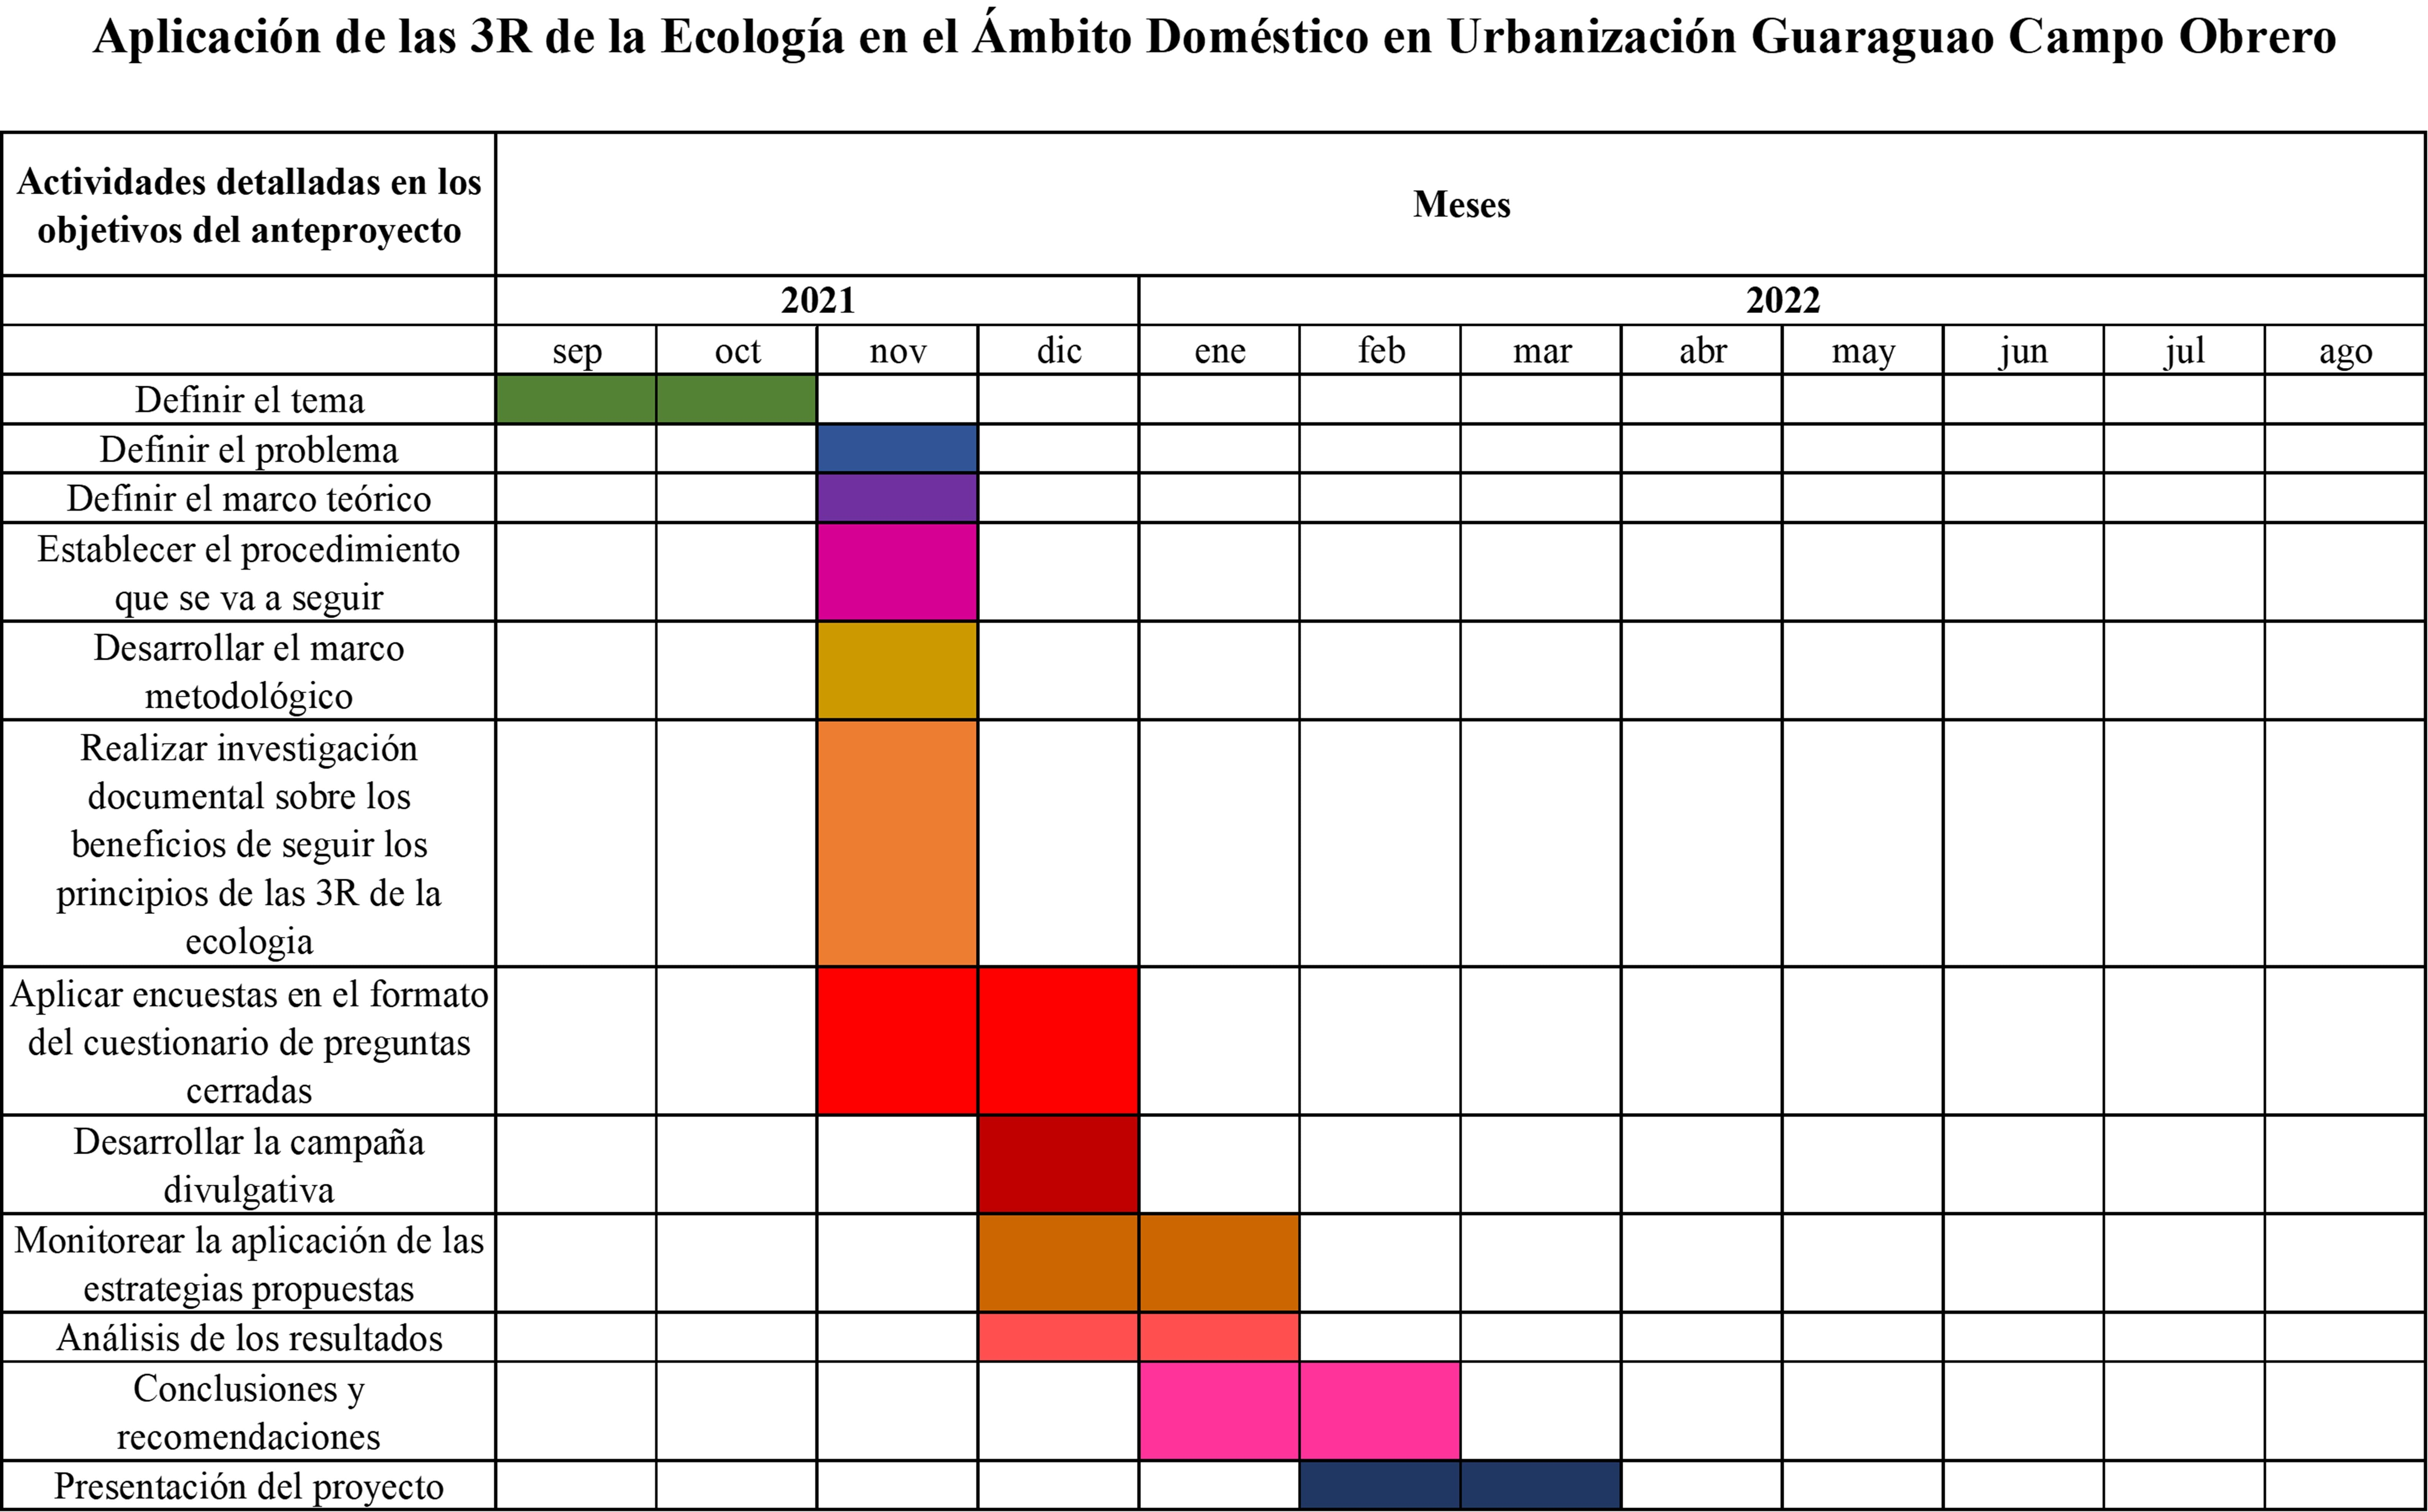
\includegraphics[width=15cm]{Media/Cronograma.jpg}
    %\caption{Cronograma de actividades formuladas en los objetivos del anteproyecto}
    \label{fig:cronograma}
\end{figure}
\begin{center} Figura 1: Cronograma de actividades detalladas en los objetivos del anteproyecto. \\Autores: Diego Ortiz y Cynthia Cataldi \end{center}

\newpage